\documentclass[UTF8]{ctexart}
%插入数学公式
\usepackage{amsmath}
\usepackage{amssymb}
\usepackage{graphicx} % 图片插入
%设置纸张和页边距 A4
\usepackage{geometry}
\geometry{papersize={21cm,29.7cm}}
\geometry{left=3.18cm,right=3.18cm,top=2.54cm,bottom=2.54cm}
% 一级标题靠左
\CTEXsetup[format={\Large\bfseries}]{section}
% 去除页眉
\pagestyle{plain}
% %设置行间距 1.5倍行距
% \usepackage{setspace}
% \onehalfspacing
%设置段间距
\addtolength{\parskip}{.4em}
\title{信号与系统课程笔记:Lecture 6}
\author{授课教师:秦雨潇 \\
笔记记录:曹时成}
\date{2023年10月11日(第六周,周三)}

\begin{document}
\maketitle
\section{课堂回顾:卷积}
1. $f(t)= \int _\mathbb{R} f(\tau ) \delta  (t-\tau  ) \,d\tau  $  \par
\quad $\mid \mid \mid $ \par
2. $f(t)=f(t)\ast \delta (t) $ \par
\quad 对于一般信号可用特殊信号表达 \par
\quad \quad $\delta (t) \ast h(t)=h(t)$ \; 对于 : \,$\delta (t) \rightarrow \boxed{h(t)}\rightarrow h(t)$ ,其中$\boxed{h(t)}$被称为“照妖镜”系统\par
\qquad \qquad \quad$\downarrow $ LTI \par
\quad \quad $f (t) \ast h(t)=y(t)$ \par

\section{信号的分解形式如何表达?}
\subsection{下面哪种特殊信号用来表达信号最好?(这里不区分离散和连续)}

(1)$\delta $函数:$\delta [k-\tau ]$ \par
\begin{figure}[h]
    \centering         %使图片居中放置
    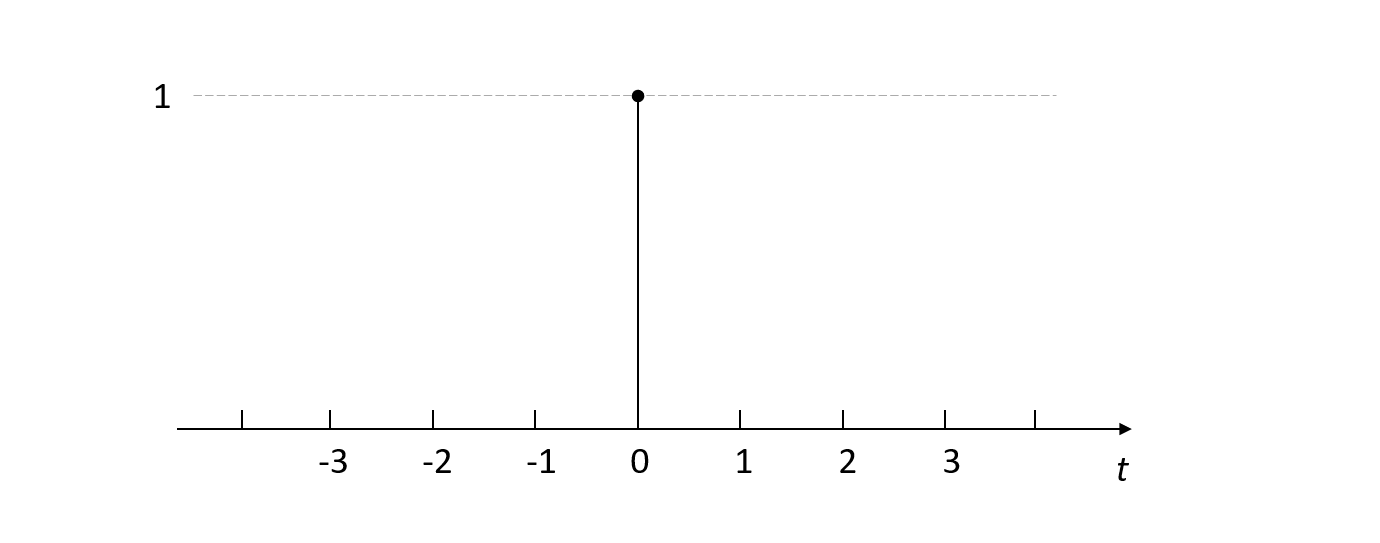
\includegraphics[scale=0.35]{1.png}      
    \caption{$\delta $ 函数信号形式}
\end{figure}
\,\par
(2)阶跃函数:$u [k-\tau ]$ \par
\begin{figure}[h]
    \centering         %使图片居中放置
    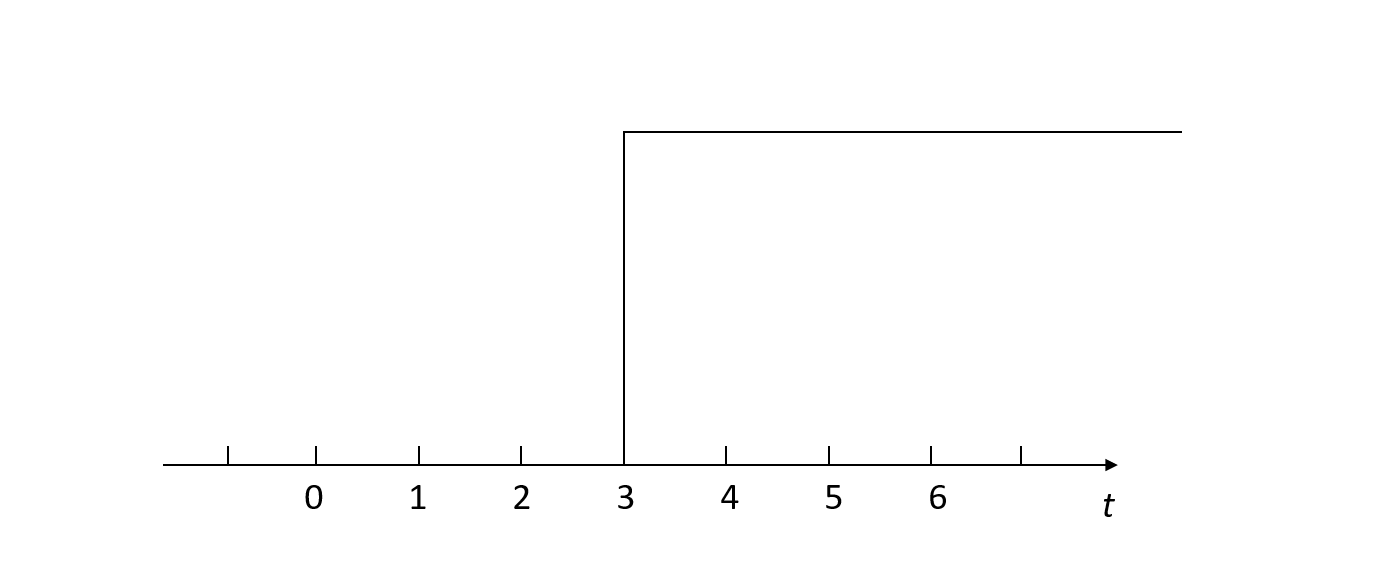
\includegraphics[scale=0.35]{2.jpg}
    \caption{阶跃函数信号形式}
\end{figure}
(3)门函数:$rect [k-\tau ]$ \par
\begin{figure}[h] 
    \centering         %使图片居中放置
    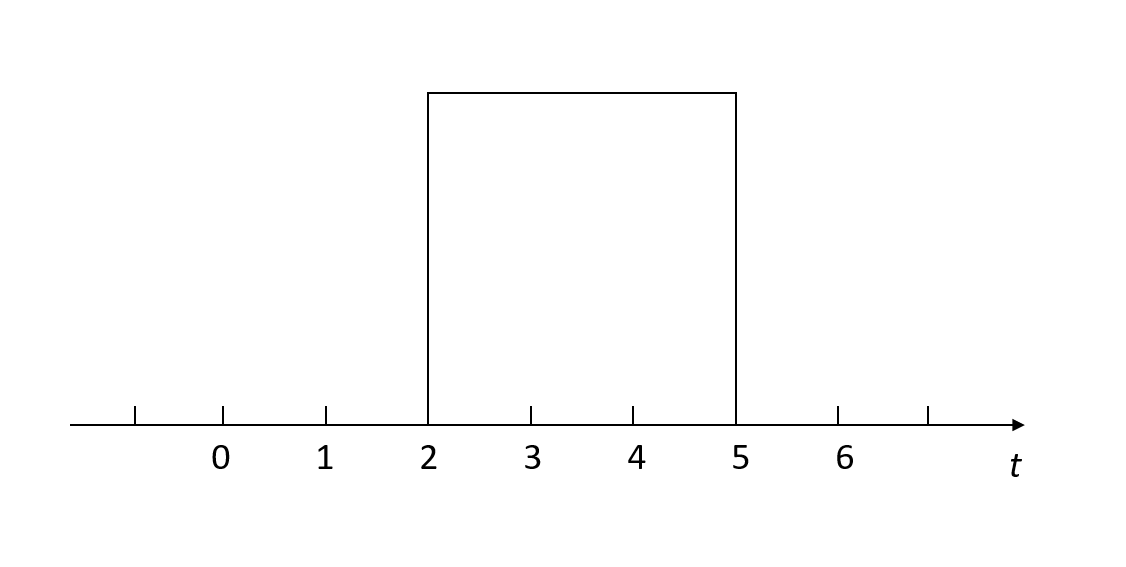
\includegraphics[scale=0.35]{3.jpg}
    \caption{门函数信号形式}
\end{figure}
(4)随机分布函数:$N(\mu ,\delta ): f(x)=\frac{1}{\sigma \sqrt{2\pi }} e^{-\frac{(x-\mu )^2}{2\sigma ^2} } $ \par
\begin{figure}[h]
    \centering         %使图片居中放置
    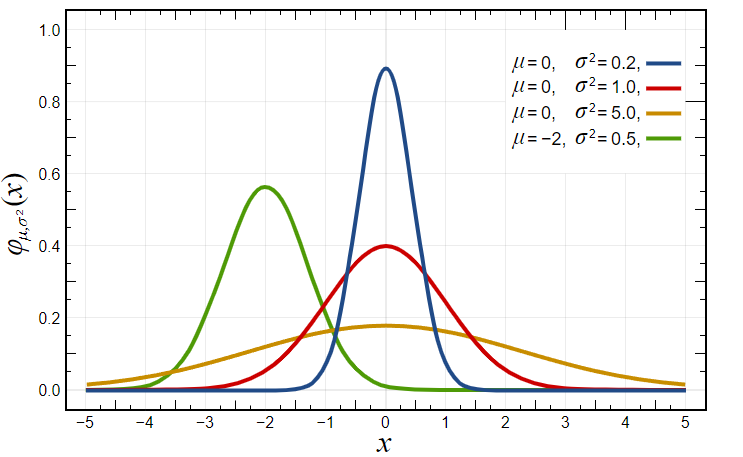
\includegraphics[scale=0.35]{4.jpg}
    \caption{随机分布函数信号形式}
\end{figure}

\subsection{Q:一个一般性的信号分解方式是什么?如何用数学语言描述?}
例如,对于一个二维信号,可以在两个维度上进行分解 \par
$\vec{f}= \left[   
    \begin{matrix}
    x \\
    y \\
    \end{matrix}
  \right]
  = x\cdot\vec{v}_x+y\cdot\vec{v}_y $
\begin{figure}[h]
    \centering         %使图片居中放置
    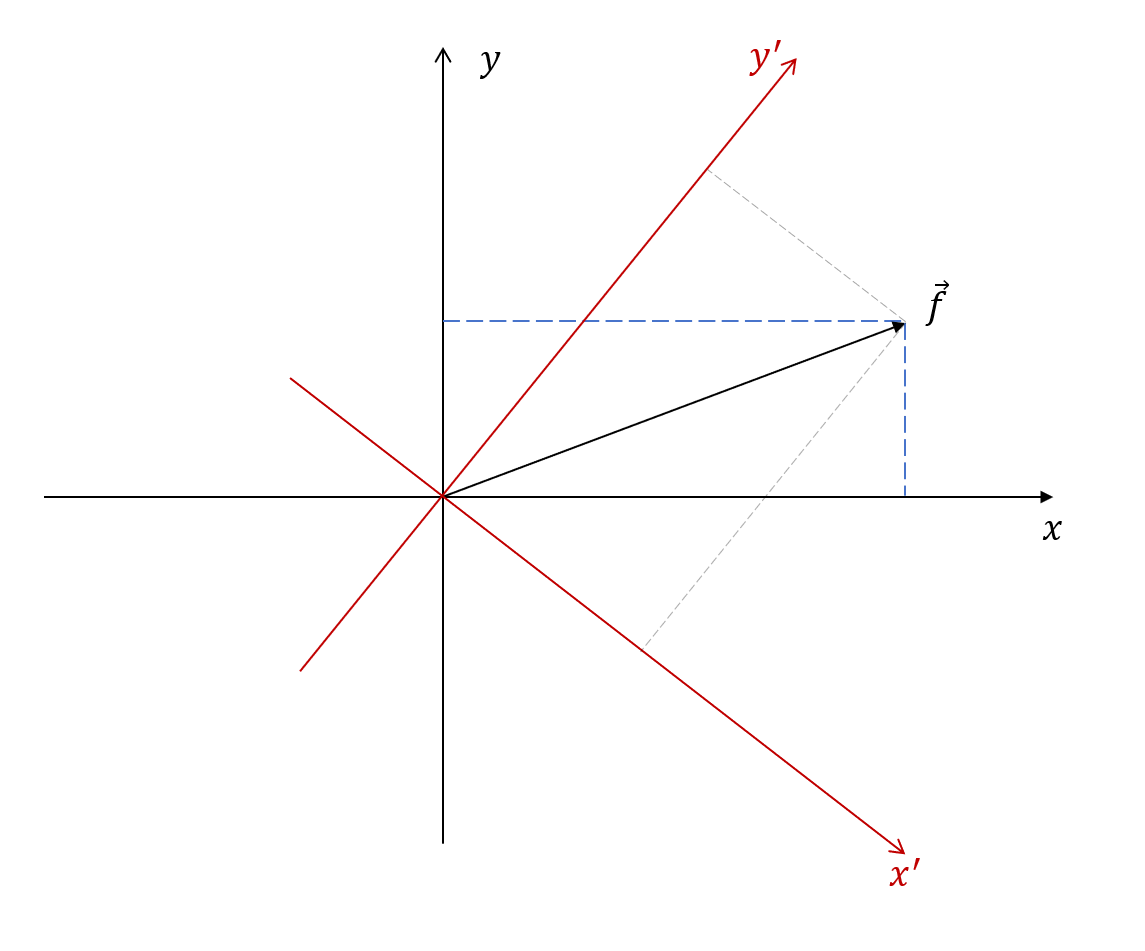
\includegraphics[scale=0.35]{5.jpg}
    \caption{$\vec{f}$在任意两个维度上进行分解}
\end{figure}
\, \par
\, \par
选择特殊信号(特殊维度)的要求: \par
(1)$\vec{v}_x\perp \vec{v}_y$ \par
(2)$\parallel \vec{v}_x\parallel = \parallel\vec{v}_y\parallel$ \par
(3)$span\{\vec{v}_x, \vec{v}_y\}  \in \mathbb{R} ^2 $ \par
此外,$\vec{f}$在维度$\vec{v}_x$上的投影$\vec{f}_x$为:\par
$\vec{f}_x= \langle \vec{f}\cdot\vec{v}_x\rangle =\| \vec{f} \Vert \cdot  \| \vec{v}_x\Vert \cdot cos\theta  $
\end{document}